\documentclass[twoside]{book}

% Packages required by doxygen
\usepackage{fixltx2e}
\usepackage{calc}
\usepackage{doxygen}
\usepackage[export]{adjustbox} % also loads graphicx
\usepackage{graphicx}
\usepackage[utf8]{inputenc}
\usepackage{makeidx}
\usepackage{multicol}
\usepackage{multirow}
\PassOptionsToPackage{warn}{textcomp}
\usepackage{textcomp}
\usepackage[nointegrals]{wasysym}
\usepackage[table]{xcolor}

% Font selection
\usepackage[T1]{fontenc}
\usepackage[scaled=.90]{helvet}
\usepackage{courier}
\usepackage{amssymb}
\usepackage{sectsty}
\renewcommand{\familydefault}{\sfdefault}
\allsectionsfont{%
  \fontseries{bc}\selectfont%
  \color{darkgray}%
}
\renewcommand{\DoxyLabelFont}{%
  \fontseries{bc}\selectfont%
  \color{darkgray}%
}
\newcommand{\+}{\discretionary{\mbox{\scriptsize$\hookleftarrow$}}{}{}}

% Page & text layout
\usepackage{geometry}
\geometry{%
  a4paper,%
  top=2.5cm,%
  bottom=2.5cm,%
  left=2.5cm,%
  right=2.5cm%
}
\tolerance=750
\hfuzz=15pt
\hbadness=750
\setlength{\emergencystretch}{15pt}
\setlength{\parindent}{0cm}
\setlength{\parskip}{3ex plus 2ex minus 2ex}
\makeatletter
\renewcommand{\paragraph}{%
  \@startsection{paragraph}{4}{0ex}{-1.0ex}{1.0ex}{%
    \normalfont\normalsize\bfseries\SS@parafont%
  }%
}
\renewcommand{\subparagraph}{%
  \@startsection{subparagraph}{5}{0ex}{-1.0ex}{1.0ex}{%
    \normalfont\normalsize\bfseries\SS@subparafont%
  }%
}
\makeatother

% Headers & footers
\usepackage{fancyhdr}
\pagestyle{fancyplain}
\fancyhead[LE]{\fancyplain{}{\bfseries\thepage}}
\fancyhead[CE]{\fancyplain{}{}}
\fancyhead[RE]{\fancyplain{}{\bfseries\leftmark}}
\fancyhead[LO]{\fancyplain{}{\bfseries\rightmark}}
\fancyhead[CO]{\fancyplain{}{}}
\fancyhead[RO]{\fancyplain{}{\bfseries\thepage}}
\fancyfoot[LE]{\fancyplain{}{}}
\fancyfoot[CE]{\fancyplain{}{}}
\fancyfoot[RE]{\fancyplain{}{\bfseries\scriptsize Generated by Doxygen }}
\fancyfoot[LO]{\fancyplain{}{\bfseries\scriptsize Generated by Doxygen }}
\fancyfoot[CO]{\fancyplain{}{}}
\fancyfoot[RO]{\fancyplain{}{}}
\renewcommand{\footrulewidth}{0.4pt}
\renewcommand{\chaptermark}[1]{%
  \markboth{#1}{}%
}
\renewcommand{\sectionmark}[1]{%
  \markright{\thesection\ #1}%
}

% Indices & bibliography
\usepackage{natbib}
\usepackage[titles]{tocloft}
\setcounter{tocdepth}{3}
\setcounter{secnumdepth}{5}
\makeindex

% Hyperlinks (required, but should be loaded last)
\usepackage{ifpdf}
\ifpdf
  \usepackage[pdftex,pagebackref=true]{hyperref}
\else
  \usepackage[ps2pdf,pagebackref=true]{hyperref}
\fi
\hypersetup{%
  colorlinks=true,%
  linkcolor=blue,%
  citecolor=blue,%
  unicode%
}

% Custom commands
\newcommand{\clearemptydoublepage}{%
  \newpage{\pagestyle{empty}\cleardoublepage}%
}

\usepackage{caption}
\captionsetup{labelsep=space,justification=centering,font={bf},singlelinecheck=off,skip=4pt,position=top}

%===== C O N T E N T S =====

\begin{document}

% Titlepage & ToC
\hypersetup{pageanchor=false,
             bookmarksnumbered=true,
             pdfencoding=unicode
            }
\pagenumbering{alph}
\begin{titlepage}
\vspace*{7cm}
\begin{center}%
{\Large A\+E\+D\+A1819\+\_\+\+Turma3\+\_\+\+G6 \\[1ex]\large 1 }\\
\vspace*{1cm}
{\large Generated by Doxygen 1.8.14}\\
\end{center}
\end{titlepage}
\clearemptydoublepage
\pagenumbering{roman}
\tableofcontents
\clearemptydoublepage
\pagenumbering{arabic}
\hypersetup{pageanchor=true}

%--- Begin generated contents ---
\chapter{Hierarchical Index}
\section{Class Hierarchy}
This inheritance list is sorted roughly, but not completely, alphabetically\+:\begin{DoxyCompactList}
\item \contentsline{section}{Bilhete}{\pageref{class_bilhete}}{}
\item \contentsline{section}{Opcao\+Invalida}{\pageref{class_opcao_invalida}}{}
\item \contentsline{section}{Posto\+De\+Venda}{\pageref{class_posto_de_venda}}{}
\begin{DoxyCompactList}
\item \contentsline{section}{Maq\+Automatica}{\pageref{class_maq_automatica}}{}
\end{DoxyCompactList}
\end{DoxyCompactList}

\chapter{Class Index}
\section{Class List}
Here are the classes, structs, unions and interfaces with brief descriptions\+:\begin{DoxyCompactList}
\item\contentsline{section}{\mbox{\hyperlink{class_bilhete}{Bilhete}} }{\pageref{class_bilhete}}{}
\item\contentsline{section}{\mbox{\hyperlink{class_maq_automatica}{Maq\+Automatica}} }{\pageref{class_maq_automatica}}{}
\item\contentsline{section}{\mbox{\hyperlink{class_opcao_invalida}{Opcao\+Invalida}} }{\pageref{class_opcao_invalida}}{}
\item\contentsline{section}{\mbox{\hyperlink{class_posto_de_venda}{Posto\+De\+Venda}} }{\pageref{class_posto_de_venda}}{}
\end{DoxyCompactList}

\chapter{Class Documentation}
\hypertarget{class_bilhete}{}\section{Bilhete Class Reference}
\label{class_bilhete}\index{Bilhete@{Bilhete}}


{\ttfamily \#include $<$Bilhete.\+h$>$}

\subsection*{Public Member Functions}
\begin{DoxyCompactItemize}
\item 
\mbox{\hyperlink{class_bilhete_a474406ccf54268b9206c936be473a15d}{Bilhete}} (cat\+\_\+zonas cat, tipo\+\_\+bilh tip, int \mbox{\hyperlink{class_bilhete_ad3dbd72118947c8ebb9d2a1a9e6bc3eb}{dia}}, int \mbox{\hyperlink{class_bilhete_ad654ce2fb56eca0738e6994774bb9d75}{mes}}, int \mbox{\hyperlink{class_bilhete_a28c57c28b91d9d751cb8292911af4b00}{ano}}, string \mbox{\hyperlink{class_bilhete_a6c473f8854c6980af895803cfe742279}{nome}}=\char`\"{}null\char`\"{}, int \mbox{\hyperlink{class_bilhete_a5cd410905c9eeb3e0281df97ddc6b69a}{idade}}=-\/1, int \mbox{\hyperlink{class_bilhete_a3272957b6efbae819c70320b40823e46}{CC}}=-\/1, string esc=\char`\"{}null\char`\"{})
\item 
string \mbox{\hyperlink{class_bilhete_ab10b04a33753b9b0f5091bb5e6f12a20}{get\+Categoria}} ()
\item 
string \mbox{\hyperlink{class_bilhete_a454736f9880f0ee44e53cca1e894df7d}{get\+Tipo}} ()
\item 
double \mbox{\hyperlink{class_bilhete_af8800b8f21428964d446d2cb0747e9d8}{get\+Preco}} ()
\item 
string \mbox{\hyperlink{class_bilhete_adf630342c192da168a75e6bc983d7801}{get\+Escola}} ()
\item 
string \mbox{\hyperlink{class_bilhete_acd970616a71c2eaf21b0d616a7a5f7aa}{get\+Nome}} ()
\item 
void \mbox{\hyperlink{class_bilhete_abae0b23c34a8538b91ea5dbd70606525}{print\+Bilhete}} ()
\item 
int \mbox{\hyperlink{class_bilhete_a328c577511937f1ab79d9e785dd18564}{get\+CC}} ()
\item 
int \mbox{\hyperlink{class_bilhete_aa63d79d55516bdb158ffc9e8abaff93c}{get\+Idade}} ()
\item 
vector$<$ int $>$ \mbox{\hyperlink{class_bilhete_a89a41aff919d6acb173acc708367f2d3}{get\+Data}} ()
\item 
bool \mbox{\hyperlink{class_bilhete_a09be5c8b845201431c4e96cc6e441f11}{operator$<$}} (const \mbox{\hyperlink{class_bilhete}{Bilhete}} \&c) const
\item 
bool \mbox{\hyperlink{class_bilhete_a3fb340596c0ab30945a1de6b691c842b}{operator$>$}} (const \mbox{\hyperlink{class_bilhete}{Bilhete}} \&c) const
\end{DoxyCompactItemize}
\subsection*{Protected Attributes}
\begin{DoxyCompactItemize}
\item 
cat\+\_\+zonas \mbox{\hyperlink{class_bilhete_a964746f80b1342fc53512073b5588c1a}{categoria}}
\item 
tipo\+\_\+bilh \mbox{\hyperlink{class_bilhete_a811d01c91c9ca7e43ca05b4de7cb053d}{tipo}}
\item 
string \mbox{\hyperlink{class_bilhete_a5129f08ea3f4b9ec1c77be2b5377c32f}{escola}}
\item 
string \mbox{\hyperlink{class_bilhete_a6c473f8854c6980af895803cfe742279}{nome}}
\item 
int \mbox{\hyperlink{class_bilhete_a3272957b6efbae819c70320b40823e46}{CC}}
\item 
int \mbox{\hyperlink{class_bilhete_a5cd410905c9eeb3e0281df97ddc6b69a}{idade}}
\item 
int \mbox{\hyperlink{class_bilhete_ad3dbd72118947c8ebb9d2a1a9e6bc3eb}{dia}}
\item 
int \mbox{\hyperlink{class_bilhete_ad654ce2fb56eca0738e6994774bb9d75}{mes}}
\item 
int \mbox{\hyperlink{class_bilhete_a28c57c28b91d9d751cb8292911af4b00}{ano}}
\end{DoxyCompactItemize}


\subsection{Detailed Description}
class \mbox{\hyperlink{class_bilhete}{Bilhete}} representa um bilhete de metro emitido, independentemente do tipo e zona 

\subsection{Constructor \& Destructor Documentation}
\mbox{\Hypertarget{class_bilhete_a474406ccf54268b9206c936be473a15d}\label{class_bilhete_a474406ccf54268b9206c936be473a15d}} 
\index{Bilhete@{Bilhete}!Bilhete@{Bilhete}}
\index{Bilhete@{Bilhete}!Bilhete@{Bilhete}}
\subsubsection{\texorpdfstring{Bilhete()}{Bilhete()}}
{\footnotesize\ttfamily Bilhete\+::\+Bilhete (\begin{DoxyParamCaption}\item[{cat\+\_\+zonas}]{cat,  }\item[{tipo\+\_\+bilh}]{tip,  }\item[{int}]{dia,  }\item[{int}]{mes,  }\item[{int}]{ano,  }\item[{string}]{nome = {\ttfamily \char`\"{}null\char`\"{}},  }\item[{int}]{idade = {\ttfamily -\/1},  }\item[{int}]{CC = {\ttfamily -\/1},  }\item[{string}]{esc = {\ttfamily \char`\"{}null\char`\"{}} }\end{DoxyParamCaption})}

construtor da class \mbox{\hyperlink{class_bilhete}{Bilhete}} 
\begin{DoxyParams}{Parameters}
{\em cat} & zona do bilhete \\
\hline
{\em tip} & tipo do bilhete \\
\hline
{\em dia} & dia de emissao do bilhete \\
\hline
{\em mes} & mes de emissao do bilhete \\
\hline
{\em ano} & ano de emissao do bilhete \\
\hline
{\em nome} & nome do comprador do bilhete (apenas para assinaturas) \\
\hline
{\em idade} & idade do comprador do bilhete (apenas para assinaturas junior, senior e estudante) \\
\hline
{\em CC} & numero do cartao de cidadao do comprador do bilhete (apenas para assinaturas junior, senior e estudante) \\
\hline
{\em esc} & escola do comprador do bilhete (apenas para assinaturas estudante) \\
\hline
\end{DoxyParams}


\subsection{Member Function Documentation}
\mbox{\Hypertarget{class_bilhete_ab10b04a33753b9b0f5091bb5e6f12a20}\label{class_bilhete_ab10b04a33753b9b0f5091bb5e6f12a20}} 
\index{Bilhete@{Bilhete}!get\+Categoria@{get\+Categoria}}
\index{get\+Categoria@{get\+Categoria}!Bilhete@{Bilhete}}
\subsubsection{\texorpdfstring{get\+Categoria()}{getCategoria()}}
{\footnotesize\ttfamily string Bilhete\+::get\+Categoria (\begin{DoxyParamCaption}{ }\end{DoxyParamCaption})}

retorna a zona do bilhete \begin{DoxyReturn}{Returns}
zona do bilhete 
\end{DoxyReturn}
\mbox{\Hypertarget{class_bilhete_a328c577511937f1ab79d9e785dd18564}\label{class_bilhete_a328c577511937f1ab79d9e785dd18564}} 
\index{Bilhete@{Bilhete}!get\+CC@{get\+CC}}
\index{get\+CC@{get\+CC}!Bilhete@{Bilhete}}
\subsubsection{\texorpdfstring{get\+C\+C()}{getCC()}}
{\footnotesize\ttfamily int Bilhete\+::get\+CC (\begin{DoxyParamCaption}{ }\end{DoxyParamCaption})}

retorna o numero do CC do comprador do bilhete \begin{DoxyReturn}{Returns}
numero do CC do comprador do bilhete 
\end{DoxyReturn}
\mbox{\Hypertarget{class_bilhete_a89a41aff919d6acb173acc708367f2d3}\label{class_bilhete_a89a41aff919d6acb173acc708367f2d3}} 
\index{Bilhete@{Bilhete}!get\+Data@{get\+Data}}
\index{get\+Data@{get\+Data}!Bilhete@{Bilhete}}
\subsubsection{\texorpdfstring{get\+Data()}{getData()}}
{\footnotesize\ttfamily vector$<$ int $>$ Bilhete\+::get\+Data (\begin{DoxyParamCaption}{ }\end{DoxyParamCaption})}

retorna a data de emissao do bilhete \begin{DoxyReturn}{Returns}
vector que contem a data de emissao do bilhete na forma \{DD,MM,A\+A\+AA\} 
\end{DoxyReturn}
\mbox{\Hypertarget{class_bilhete_adf630342c192da168a75e6bc983d7801}\label{class_bilhete_adf630342c192da168a75e6bc983d7801}} 
\index{Bilhete@{Bilhete}!get\+Escola@{get\+Escola}}
\index{get\+Escola@{get\+Escola}!Bilhete@{Bilhete}}
\subsubsection{\texorpdfstring{get\+Escola()}{getEscola()}}
{\footnotesize\ttfamily string Bilhete\+::get\+Escola (\begin{DoxyParamCaption}{ }\end{DoxyParamCaption})}

retorna a escola do comprador do bilhete \begin{DoxyReturn}{Returns}
escola do comprador do bilhete 
\end{DoxyReturn}
\mbox{\Hypertarget{class_bilhete_aa63d79d55516bdb158ffc9e8abaff93c}\label{class_bilhete_aa63d79d55516bdb158ffc9e8abaff93c}} 
\index{Bilhete@{Bilhete}!get\+Idade@{get\+Idade}}
\index{get\+Idade@{get\+Idade}!Bilhete@{Bilhete}}
\subsubsection{\texorpdfstring{get\+Idade()}{getIdade()}}
{\footnotesize\ttfamily int Bilhete\+::get\+Idade (\begin{DoxyParamCaption}{ }\end{DoxyParamCaption})}

retorna a idade do comprador do bilhete \begin{DoxyReturn}{Returns}
idade do comprador do bilhete 
\end{DoxyReturn}
\mbox{\Hypertarget{class_bilhete_acd970616a71c2eaf21b0d616a7a5f7aa}\label{class_bilhete_acd970616a71c2eaf21b0d616a7a5f7aa}} 
\index{Bilhete@{Bilhete}!get\+Nome@{get\+Nome}}
\index{get\+Nome@{get\+Nome}!Bilhete@{Bilhete}}
\subsubsection{\texorpdfstring{get\+Nome()}{getNome()}}
{\footnotesize\ttfamily string Bilhete\+::get\+Nome (\begin{DoxyParamCaption}{ }\end{DoxyParamCaption})}

retorna o nome do comprador do bilhete \begin{DoxyReturn}{Returns}
nome do comprador do bilhete 
\end{DoxyReturn}
\mbox{\Hypertarget{class_bilhete_af8800b8f21428964d446d2cb0747e9d8}\label{class_bilhete_af8800b8f21428964d446d2cb0747e9d8}} 
\index{Bilhete@{Bilhete}!get\+Preco@{get\+Preco}}
\index{get\+Preco@{get\+Preco}!Bilhete@{Bilhete}}
\subsubsection{\texorpdfstring{get\+Preco()}{getPreco()}}
{\footnotesize\ttfamily double Bilhete\+::get\+Preco (\begin{DoxyParamCaption}{ }\end{DoxyParamCaption})}

retorna o preco do bilhete \begin{DoxyReturn}{Returns}
preco do bilhete 
\end{DoxyReturn}
\mbox{\Hypertarget{class_bilhete_a454736f9880f0ee44e53cca1e894df7d}\label{class_bilhete_a454736f9880f0ee44e53cca1e894df7d}} 
\index{Bilhete@{Bilhete}!get\+Tipo@{get\+Tipo}}
\index{get\+Tipo@{get\+Tipo}!Bilhete@{Bilhete}}
\subsubsection{\texorpdfstring{get\+Tipo()}{getTipo()}}
{\footnotesize\ttfamily string Bilhete\+::get\+Tipo (\begin{DoxyParamCaption}{ }\end{DoxyParamCaption})}

retorna o tipo do bilhete \begin{DoxyReturn}{Returns}
tipo do bilhete 
\end{DoxyReturn}
\mbox{\Hypertarget{class_bilhete_a09be5c8b845201431c4e96cc6e441f11}\label{class_bilhete_a09be5c8b845201431c4e96cc6e441f11}} 
\index{Bilhete@{Bilhete}!operator$<$@{operator$<$}}
\index{operator$<$@{operator$<$}!Bilhete@{Bilhete}}
\subsubsection{\texorpdfstring{operator$<$()}{operator<()}}
{\footnotesize\ttfamily bool Bilhete\+::operator$<$ (\begin{DoxyParamCaption}\item[{const \mbox{\hyperlink{class_bilhete}{Bilhete}} \&}]{c }\end{DoxyParamCaption}) const}

retorna true se o argumento da esquerda for menor cronologicamente que o da direita \mbox{\Hypertarget{class_bilhete_a3fb340596c0ab30945a1de6b691c842b}\label{class_bilhete_a3fb340596c0ab30945a1de6b691c842b}} 
\index{Bilhete@{Bilhete}!operator$>$@{operator$>$}}
\index{operator$>$@{operator$>$}!Bilhete@{Bilhete}}
\subsubsection{\texorpdfstring{operator$>$()}{operator>()}}
{\footnotesize\ttfamily bool Bilhete\+::operator$>$ (\begin{DoxyParamCaption}\item[{const \mbox{\hyperlink{class_bilhete}{Bilhete}} \&}]{c }\end{DoxyParamCaption}) const}

retorna true se o argumento da esquerda for maior cronologicamente que o da direita \mbox{\Hypertarget{class_bilhete_abae0b23c34a8538b91ea5dbd70606525}\label{class_bilhete_abae0b23c34a8538b91ea5dbd70606525}} 
\index{Bilhete@{Bilhete}!print\+Bilhete@{print\+Bilhete}}
\index{print\+Bilhete@{print\+Bilhete}!Bilhete@{Bilhete}}
\subsubsection{\texorpdfstring{print\+Bilhete()}{printBilhete()}}
{\footnotesize\ttfamily void Bilhete\+::print\+Bilhete (\begin{DoxyParamCaption}{ }\end{DoxyParamCaption})}

imprime no ecra todos os atributos do bilhete 

\subsection{Member Data Documentation}
\mbox{\Hypertarget{class_bilhete_a28c57c28b91d9d751cb8292911af4b00}\label{class_bilhete_a28c57c28b91d9d751cb8292911af4b00}} 
\index{Bilhete@{Bilhete}!ano@{ano}}
\index{ano@{ano}!Bilhete@{Bilhete}}
\subsubsection{\texorpdfstring{ano}{ano}}
{\footnotesize\ttfamily int Bilhete\+::ano\hspace{0.3cm}{\ttfamily [protected]}}

ano de emissao do bilhete \mbox{\Hypertarget{class_bilhete_a964746f80b1342fc53512073b5588c1a}\label{class_bilhete_a964746f80b1342fc53512073b5588c1a}} 
\index{Bilhete@{Bilhete}!categoria@{categoria}}
\index{categoria@{categoria}!Bilhete@{Bilhete}}
\subsubsection{\texorpdfstring{categoria}{categoria}}
{\footnotesize\ttfamily cat\+\_\+zonas Bilhete\+::categoria\hspace{0.3cm}{\ttfamily [protected]}}

zona para a qual o bilhete foi comprado \mbox{\Hypertarget{class_bilhete_a3272957b6efbae819c70320b40823e46}\label{class_bilhete_a3272957b6efbae819c70320b40823e46}} 
\index{Bilhete@{Bilhete}!CC@{CC}}
\index{CC@{CC}!Bilhete@{Bilhete}}
\subsubsection{\texorpdfstring{CC}{CC}}
{\footnotesize\ttfamily int Bilhete\+::\+CC\hspace{0.3cm}{\ttfamily [protected]}}

numero do CC do assinante (-\/1 se o bilhete nao for assinatura junior, senior ou estudante) \mbox{\Hypertarget{class_bilhete_ad3dbd72118947c8ebb9d2a1a9e6bc3eb}\label{class_bilhete_ad3dbd72118947c8ebb9d2a1a9e6bc3eb}} 
\index{Bilhete@{Bilhete}!dia@{dia}}
\index{dia@{dia}!Bilhete@{Bilhete}}
\subsubsection{\texorpdfstring{dia}{dia}}
{\footnotesize\ttfamily int Bilhete\+::dia\hspace{0.3cm}{\ttfamily [protected]}}

$<$ dia de emissao do bilhete \mbox{\Hypertarget{class_bilhete_a5129f08ea3f4b9ec1c77be2b5377c32f}\label{class_bilhete_a5129f08ea3f4b9ec1c77be2b5377c32f}} 
\index{Bilhete@{Bilhete}!escola@{escola}}
\index{escola@{escola}!Bilhete@{Bilhete}}
\subsubsection{\texorpdfstring{escola}{escola}}
{\footnotesize\ttfamily string Bilhete\+::escola\hspace{0.3cm}{\ttfamily [protected]}}

escola do assinante ( \char`\"{}null\char`\"{} se o bilhete nao for do tipo assinatura estudante) \mbox{\Hypertarget{class_bilhete_a5cd410905c9eeb3e0281df97ddc6b69a}\label{class_bilhete_a5cd410905c9eeb3e0281df97ddc6b69a}} 
\index{Bilhete@{Bilhete}!idade@{idade}}
\index{idade@{idade}!Bilhete@{Bilhete}}
\subsubsection{\texorpdfstring{idade}{idade}}
{\footnotesize\ttfamily int Bilhete\+::idade\hspace{0.3cm}{\ttfamily [protected]}}

idade do assinante (-\/1 se o bilhete nao for assinatura junior, senior ou estudante) \mbox{\Hypertarget{class_bilhete_ad654ce2fb56eca0738e6994774bb9d75}\label{class_bilhete_ad654ce2fb56eca0738e6994774bb9d75}} 
\index{Bilhete@{Bilhete}!mes@{mes}}
\index{mes@{mes}!Bilhete@{Bilhete}}
\subsubsection{\texorpdfstring{mes}{mes}}
{\footnotesize\ttfamily int Bilhete\+::mes\hspace{0.3cm}{\ttfamily [protected]}}

$<$ mes de emissao do bilhete \mbox{\Hypertarget{class_bilhete_a6c473f8854c6980af895803cfe742279}\label{class_bilhete_a6c473f8854c6980af895803cfe742279}} 
\index{Bilhete@{Bilhete}!nome@{nome}}
\index{nome@{nome}!Bilhete@{Bilhete}}
\subsubsection{\texorpdfstring{nome}{nome}}
{\footnotesize\ttfamily string Bilhete\+::nome\hspace{0.3cm}{\ttfamily [protected]}}

nome do assinante (\char`\"{}null\char`\"{} se o bilhete nao for de um tipo assinatura) \mbox{\Hypertarget{class_bilhete_a811d01c91c9ca7e43ca05b4de7cb053d}\label{class_bilhete_a811d01c91c9ca7e43ca05b4de7cb053d}} 
\index{Bilhete@{Bilhete}!tipo@{tipo}}
\index{tipo@{tipo}!Bilhete@{Bilhete}}
\subsubsection{\texorpdfstring{tipo}{tipo}}
{\footnotesize\ttfamily tipo\+\_\+bilh Bilhete\+::tipo\hspace{0.3cm}{\ttfamily [protected]}}

tipo do bilhete 

The documentation for this class was generated from the following files\+:\begin{DoxyCompactItemize}
\item 
D\+:/\+Moon\+\_\+\+Over\+\_\+\+Sun/\+A\+E\+D\+A1819\+\_\+\+Turma3\+\_\+\+G6/src/Bilhete.\+h\item 
D\+:/\+Moon\+\_\+\+Over\+\_\+\+Sun/\+A\+E\+D\+A1819\+\_\+\+Turma3\+\_\+\+G6/src/Bilhete.\+cpp\end{DoxyCompactItemize}

\hypertarget{class_maq_automatica}{}\section{Maq\+Automatica Class Reference}
\label{class_maq_automatica}\index{Maq\+Automatica@{Maq\+Automatica}}


{\ttfamily \#include $<$Posto\+De\+Venda.\+h$>$}

Inheritance diagram for Maq\+Automatica\+:\begin{figure}[H]
\begin{center}
\leavevmode
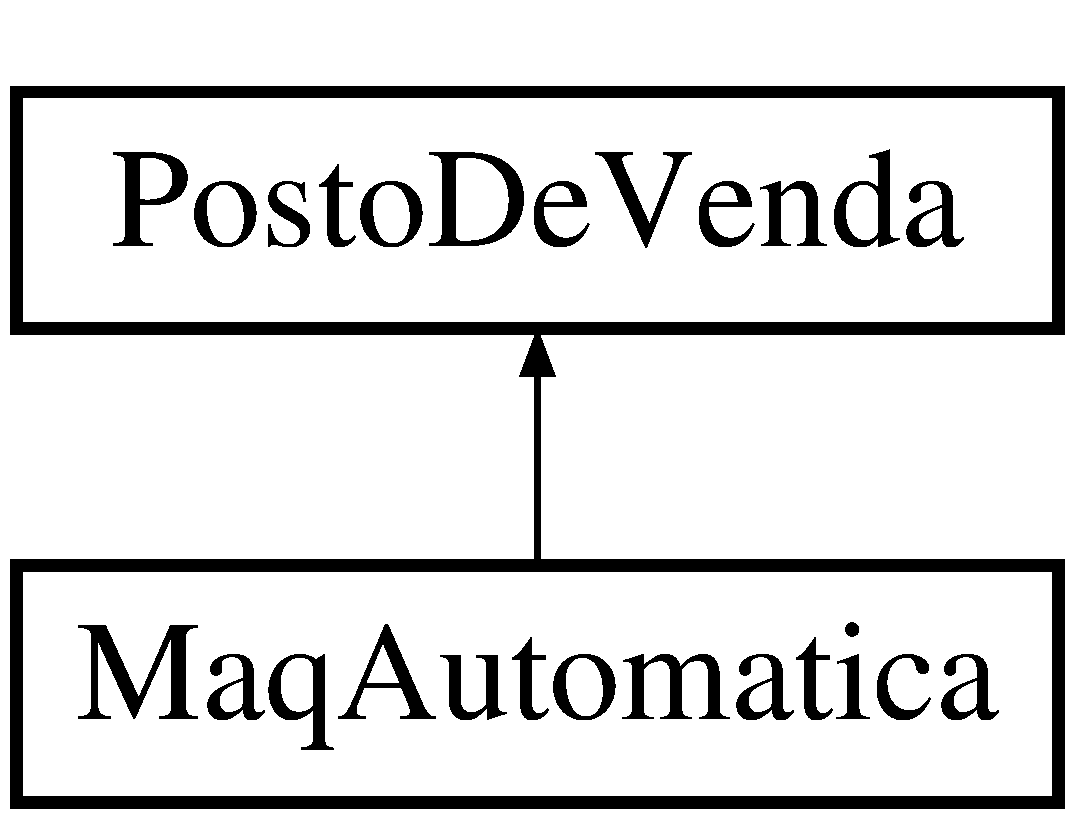
\includegraphics[height=2.000000cm]{class_maq_automatica}
\end{center}
\end{figure}
\subsection*{Public Member Functions}
\begin{DoxyCompactItemize}
\item 
\mbox{\hyperlink{class_maq_automatica_a66ad0469b8f045078f67d4b7a73fc20f}{Maq\+Automatica}} (string loc)
\item 
void \mbox{\hyperlink{class_maq_automatica_abd628f63dcfc0e9f023b84f187ff3602}{emite\+Bilhete}} (cat\+\_\+zonas cat, tipo\+\_\+bilh tip, int dia, int mes, int ano)
\end{DoxyCompactItemize}
\subsection*{Additional Inherited Members}


\subsection{Detailed Description}
class \mbox{\hyperlink{class_maq_automatica}{Maq\+Automatica}} versao simplificada de \mbox{\hyperlink{class_posto_de_venda}{Posto\+De\+Venda}} que nao emite bilhetes assinatura 

\subsection{Constructor \& Destructor Documentation}
\mbox{\Hypertarget{class_maq_automatica_a66ad0469b8f045078f67d4b7a73fc20f}\label{class_maq_automatica_a66ad0469b8f045078f67d4b7a73fc20f}} 
\index{Maq\+Automatica@{Maq\+Automatica}!Maq\+Automatica@{Maq\+Automatica}}
\index{Maq\+Automatica@{Maq\+Automatica}!Maq\+Automatica@{Maq\+Automatica}}
\subsubsection{\texorpdfstring{Maq\+Automatica()}{MaqAutomatica()}}
{\footnotesize\ttfamily Maq\+Automatica\+::\+Maq\+Automatica (\begin{DoxyParamCaption}\item[{string}]{loc }\end{DoxyParamCaption})}

construtor da class \mbox{\hyperlink{class_maq_automatica}{Maq\+Automatica}} 
\begin{DoxyParams}{Parameters}
{\em loc} & localizacao da maquina \\
\hline
\end{DoxyParams}


\subsection{Member Function Documentation}
\mbox{\Hypertarget{class_maq_automatica_abd628f63dcfc0e9f023b84f187ff3602}\label{class_maq_automatica_abd628f63dcfc0e9f023b84f187ff3602}} 
\index{Maq\+Automatica@{Maq\+Automatica}!emite\+Bilhete@{emite\+Bilhete}}
\index{emite\+Bilhete@{emite\+Bilhete}!Maq\+Automatica@{Maq\+Automatica}}
\subsubsection{\texorpdfstring{emite\+Bilhete()}{emiteBilhete()}}
{\footnotesize\ttfamily void Maq\+Automatica\+::emite\+Bilhete (\begin{DoxyParamCaption}\item[{cat\+\_\+zonas}]{cat,  }\item[{tipo\+\_\+bilh}]{tip,  }\item[{int}]{dia,  }\item[{int}]{mes,  }\item[{int}]{ano }\end{DoxyParamCaption})}

funcao que cria um bilhete e o coloca no vetor de bilhetes 
\begin{DoxyParams}{Parameters}
{\em cat} & zona do bilhete \\
\hline
{\em tip} & tipo do bilhete \\
\hline
{\em dia} & dia de emissao do bilhete \\
\hline
{\em mes} & mes de emissao do bilhete \\
\hline
{\em ano} & ano de emissao do bilhete \\
\hline
\end{DoxyParams}


The documentation for this class was generated from the following files\+:\begin{DoxyCompactItemize}
\item 
D\+:/\+Moon\+\_\+\+Over\+\_\+\+Sun/\+A\+E\+D\+A1819\+\_\+\+Turma3\+\_\+\+G6/src/Posto\+De\+Venda.\+h\item 
D\+:/\+Moon\+\_\+\+Over\+\_\+\+Sun/\+A\+E\+D\+A1819\+\_\+\+Turma3\+\_\+\+G6/src/Posto\+De\+Venda.\+cpp\end{DoxyCompactItemize}

\hypertarget{class_opcao_invalida}{}\section{Opcao\+Invalida Class Reference}
\label{class_opcao_invalida}\index{Opcao\+Invalida@{Opcao\+Invalida}}


\subsection{Detailed Description}
class excecao para inputs invalidos 

The documentation for this class was generated from the following file\+:\begin{DoxyCompactItemize}
\item 
D\+:/\+Moon\+\_\+\+Over\+\_\+\+Sun/\+A\+E\+D\+A1819\+\_\+\+Turma3\+\_\+\+G6/src/main.\+cpp\end{DoxyCompactItemize}

\hypertarget{class_posto_de_venda}{}\section{Posto\+De\+Venda Class Reference}
\label{class_posto_de_venda}\index{Posto\+De\+Venda@{Posto\+De\+Venda}}


{\ttfamily \#include $<$Posto\+De\+Venda.\+h$>$}

Inheritance diagram for Posto\+De\+Venda\+:\begin{figure}[H]
\begin{center}
\leavevmode
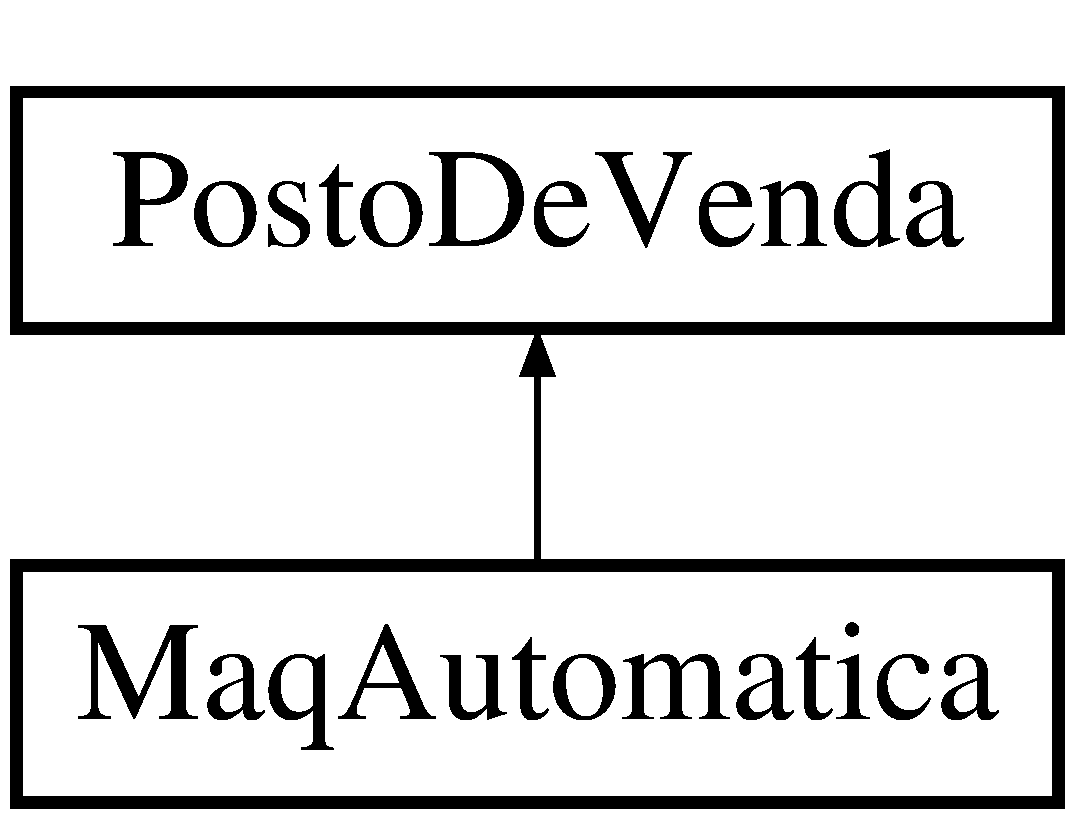
\includegraphics[height=2.000000cm]{class_posto_de_venda}
\end{center}
\end{figure}
\subsection*{Public Member Functions}
\begin{DoxyCompactItemize}
\item 
\mbox{\hyperlink{class_posto_de_venda_a38d7208ee6ce358f68a93962f26cc0d2}{Posto\+De\+Venda}} (string loc)
\item 
virtual \mbox{\hyperlink{class_posto_de_venda_a1dd82f94c0f855c241a8cf7746965352}{$\sim$\+Posto\+De\+Venda}} ()
\item 
vector$<$ \mbox{\hyperlink{class_bilhete}{Bilhete}} $>$ \mbox{\hyperlink{class_posto_de_venda_ada877eae009390d451031c273cf79b3c}{get\+Bilhetes}} ()
\item 
virtual void \mbox{\hyperlink{class_posto_de_venda_a7f8bb1189135f8e56e468b4ead96d687}{emite\+Bilhete}} (cat\+\_\+zonas cat, tipo\+\_\+bilh tip, int dia, int mes, int ano, string nome=\char`\"{}null\char`\"{}, int idade=-\/1, int CC=-\/1, string esc=\char`\"{}null\char`\"{})
\item 
void \mbox{\hyperlink{class_posto_de_venda_aaa946b8d9f379973fa3d2ce0b76f9c5a}{print\+Bilhetes}} (bool print\+Period)
\item 
int \mbox{\hyperlink{class_posto_de_venda_a92123fdb7770ce4e9f391ce652f7f05d}{numero\+Bilhetes}} ()
\item 
int \mbox{\hyperlink{class_posto_de_venda_af08c849d41568046be954beafd883336}{numero\+Bilhetes}} (cat\+\_\+zonas cat)
\item 
int \mbox{\hyperlink{class_posto_de_venda_af040c9193cb3570c6939adbb54fbe745}{numero\+Bilhetes}} (tipo\+\_\+bilh tip)
\item 
string \mbox{\hyperlink{class_posto_de_venda_a3af556f26b273caa539a5dd2c2422020}{get\+Localizacao}} ()
\item 
void \mbox{\hyperlink{class_posto_de_venda_a1bbfe0ac44c5cd095b7030b41ef3a606}{ordena\+Bilhetes}} ()
\end{DoxyCompactItemize}
\subsection*{Protected Attributes}
\begin{DoxyCompactItemize}
\item 
string \mbox{\hyperlink{class_posto_de_venda_a17c40dce2788e8b5263ea344fa742ec9}{localizacao}}
\item 
vector$<$ \mbox{\hyperlink{class_bilhete}{Bilhete}} $>$ \mbox{\hyperlink{class_posto_de_venda_ad17c54241efdb395d97cd6e205034b1d}{bilhetes\+\_\+emitidos}}
\end{DoxyCompactItemize}


\subsection{Detailed Description}
class \mbox{\hyperlink{class_posto_de_venda}{Posto\+De\+Venda}} inclui localizacao do posto e um vetor de bilhetes emitidos. 

\subsection{Constructor \& Destructor Documentation}
\mbox{\Hypertarget{class_posto_de_venda_a38d7208ee6ce358f68a93962f26cc0d2}\label{class_posto_de_venda_a38d7208ee6ce358f68a93962f26cc0d2}} 
\index{Posto\+De\+Venda@{Posto\+De\+Venda}!Posto\+De\+Venda@{Posto\+De\+Venda}}
\index{Posto\+De\+Venda@{Posto\+De\+Venda}!Posto\+De\+Venda@{Posto\+De\+Venda}}
\subsubsection{\texorpdfstring{Posto\+De\+Venda()}{PostoDeVenda()}}
{\footnotesize\ttfamily Posto\+De\+Venda\+::\+Posto\+De\+Venda (\begin{DoxyParamCaption}\item[{string}]{loc }\end{DoxyParamCaption})}

construtor da classe \mbox{\hyperlink{class_posto_de_venda}{Posto\+De\+Venda}} 
\begin{DoxyParams}{Parameters}
{\em loc} & localizacao do posto \\
\hline
\end{DoxyParams}
\mbox{\Hypertarget{class_posto_de_venda_a1dd82f94c0f855c241a8cf7746965352}\label{class_posto_de_venda_a1dd82f94c0f855c241a8cf7746965352}} 
\index{Posto\+De\+Venda@{Posto\+De\+Venda}!````~Posto\+De\+Venda@{$\sim$\+Posto\+De\+Venda}}
\index{````~Posto\+De\+Venda@{$\sim$\+Posto\+De\+Venda}!Posto\+De\+Venda@{Posto\+De\+Venda}}
\subsubsection{\texorpdfstring{$\sim$\+Posto\+De\+Venda()}{~PostoDeVenda()}}
{\footnotesize\ttfamily virtual Posto\+De\+Venda\+::$\sim$\+Posto\+De\+Venda (\begin{DoxyParamCaption}{ }\end{DoxyParamCaption})\hspace{0.3cm}{\ttfamily [inline]}, {\ttfamily [virtual]}}

destrutor da classe \mbox{\hyperlink{class_posto_de_venda}{Posto\+De\+Venda}} 

\subsection{Member Function Documentation}
\mbox{\Hypertarget{class_posto_de_venda_a7f8bb1189135f8e56e468b4ead96d687}\label{class_posto_de_venda_a7f8bb1189135f8e56e468b4ead96d687}} 
\index{Posto\+De\+Venda@{Posto\+De\+Venda}!emite\+Bilhete@{emite\+Bilhete}}
\index{emite\+Bilhete@{emite\+Bilhete}!Posto\+De\+Venda@{Posto\+De\+Venda}}
\subsubsection{\texorpdfstring{emite\+Bilhete()}{emiteBilhete()}}
{\footnotesize\ttfamily void Posto\+De\+Venda\+::emite\+Bilhete (\begin{DoxyParamCaption}\item[{cat\+\_\+zonas}]{cat,  }\item[{tipo\+\_\+bilh}]{tip,  }\item[{int}]{dia,  }\item[{int}]{mes,  }\item[{int}]{ano,  }\item[{string}]{nome = {\ttfamily \char`\"{}null\char`\"{}},  }\item[{int}]{idade = {\ttfamily -\/1},  }\item[{int}]{CC = {\ttfamily -\/1},  }\item[{string}]{esc = {\ttfamily \char`\"{}null\char`\"{}} }\end{DoxyParamCaption})\hspace{0.3cm}{\ttfamily [virtual]}}

funcao que cria um bilhete e o coloca no vetor de bilhetes 
\begin{DoxyParams}{Parameters}
{\em cat} & zona do bilhete \\
\hline
{\em tip} & tipo do bilhete \\
\hline
{\em dia} & dia de emissao do bilhete \\
\hline
{\em mes} & mes de emissao do bilhete \\
\hline
{\em ano} & ano de emissao do bilhete \\
\hline
{\em nome} & nome do comprador do bilhete (apenas para assinaturas) \\
\hline
{\em idade} & idade do comprador do bilhete (apenas para assinaturas junior, senior e estudante) \\
\hline
{\em CC} & numero do cartao de cidadao do comprador do bilhete (apenas para assinaturas junior, senior e estudante) \\
\hline
{\em esc} & escola do comprador do bilhete (apenas para assinaturas estudante) \\
\hline
\end{DoxyParams}
\mbox{\Hypertarget{class_posto_de_venda_ada877eae009390d451031c273cf79b3c}\label{class_posto_de_venda_ada877eae009390d451031c273cf79b3c}} 
\index{Posto\+De\+Venda@{Posto\+De\+Venda}!get\+Bilhetes@{get\+Bilhetes}}
\index{get\+Bilhetes@{get\+Bilhetes}!Posto\+De\+Venda@{Posto\+De\+Venda}}
\subsubsection{\texorpdfstring{get\+Bilhetes()}{getBilhetes()}}
{\footnotesize\ttfamily vector$<$ \mbox{\hyperlink{class_bilhete}{Bilhete}} $>$ Posto\+De\+Venda\+::get\+Bilhetes (\begin{DoxyParamCaption}{ }\end{DoxyParamCaption})}

funcao que retorna os bilhetes emitidos pelo posto \begin{DoxyReturn}{Returns}
vetor de bilhetes emitidos 
\end{DoxyReturn}
\mbox{\Hypertarget{class_posto_de_venda_a3af556f26b273caa539a5dd2c2422020}\label{class_posto_de_venda_a3af556f26b273caa539a5dd2c2422020}} 
\index{Posto\+De\+Venda@{Posto\+De\+Venda}!get\+Localizacao@{get\+Localizacao}}
\index{get\+Localizacao@{get\+Localizacao}!Posto\+De\+Venda@{Posto\+De\+Venda}}
\subsubsection{\texorpdfstring{get\+Localizacao()}{getLocalizacao()}}
{\footnotesize\ttfamily string Posto\+De\+Venda\+::get\+Localizacao (\begin{DoxyParamCaption}{ }\end{DoxyParamCaption})}

retorna a localizacao do posto \begin{DoxyReturn}{Returns}
localizacao do posto 
\end{DoxyReturn}
\mbox{\Hypertarget{class_posto_de_venda_a92123fdb7770ce4e9f391ce652f7f05d}\label{class_posto_de_venda_a92123fdb7770ce4e9f391ce652f7f05d}} 
\index{Posto\+De\+Venda@{Posto\+De\+Venda}!numero\+Bilhetes@{numero\+Bilhetes}}
\index{numero\+Bilhetes@{numero\+Bilhetes}!Posto\+De\+Venda@{Posto\+De\+Venda}}
\subsubsection{\texorpdfstring{numero\+Bilhetes()}{numeroBilhetes()}\hspace{0.1cm}{\footnotesize\ttfamily [1/3]}}
{\footnotesize\ttfamily int Posto\+De\+Venda\+::numero\+Bilhetes (\begin{DoxyParamCaption}{ }\end{DoxyParamCaption})}

retorna o numero total de bilhetes emitidos por este posto \begin{DoxyReturn}{Returns}
numero de bilhetes emitidos 
\end{DoxyReturn}
\mbox{\Hypertarget{class_posto_de_venda_af08c849d41568046be954beafd883336}\label{class_posto_de_venda_af08c849d41568046be954beafd883336}} 
\index{Posto\+De\+Venda@{Posto\+De\+Venda}!numero\+Bilhetes@{numero\+Bilhetes}}
\index{numero\+Bilhetes@{numero\+Bilhetes}!Posto\+De\+Venda@{Posto\+De\+Venda}}
\subsubsection{\texorpdfstring{numero\+Bilhetes()}{numeroBilhetes()}\hspace{0.1cm}{\footnotesize\ttfamily [2/3]}}
{\footnotesize\ttfamily int Posto\+De\+Venda\+::numero\+Bilhetes (\begin{DoxyParamCaption}\item[{cat\+\_\+zonas}]{cat }\end{DoxyParamCaption})}

retorna o numero de bilhetes de uma zona emitidos por este posto 
\begin{DoxyParams}{Parameters}
{\em cat} & zona cujos bilhetes ser�o contados \\
\hline
\end{DoxyParams}
\begin{DoxyReturn}{Returns}
numero de bilhetes da zona escolhida emitidos 
\end{DoxyReturn}
\mbox{\Hypertarget{class_posto_de_venda_af040c9193cb3570c6939adbb54fbe745}\label{class_posto_de_venda_af040c9193cb3570c6939adbb54fbe745}} 
\index{Posto\+De\+Venda@{Posto\+De\+Venda}!numero\+Bilhetes@{numero\+Bilhetes}}
\index{numero\+Bilhetes@{numero\+Bilhetes}!Posto\+De\+Venda@{Posto\+De\+Venda}}
\subsubsection{\texorpdfstring{numero\+Bilhetes()}{numeroBilhetes()}\hspace{0.1cm}{\footnotesize\ttfamily [3/3]}}
{\footnotesize\ttfamily int Posto\+De\+Venda\+::numero\+Bilhetes (\begin{DoxyParamCaption}\item[{tipo\+\_\+bilh}]{tip }\end{DoxyParamCaption})}

retorna o numero de bilhetes de um tipo emitidos por este posto 
\begin{DoxyParams}{Parameters}
{\em tip} & tipo cujos bilhetes ser�o contados \\
\hline
\end{DoxyParams}
\begin{DoxyReturn}{Returns}
numero de bilhetes do tipo escolhido emitidos 
\end{DoxyReturn}
\mbox{\Hypertarget{class_posto_de_venda_a1bbfe0ac44c5cd095b7030b41ef3a606}\label{class_posto_de_venda_a1bbfe0ac44c5cd095b7030b41ef3a606}} 
\index{Posto\+De\+Venda@{Posto\+De\+Venda}!ordena\+Bilhetes@{ordena\+Bilhetes}}
\index{ordena\+Bilhetes@{ordena\+Bilhetes}!Posto\+De\+Venda@{Posto\+De\+Venda}}
\subsubsection{\texorpdfstring{ordena\+Bilhetes()}{ordenaBilhetes()}}
{\footnotesize\ttfamily void Posto\+De\+Venda\+::ordena\+Bilhetes (\begin{DoxyParamCaption}{ }\end{DoxyParamCaption})}

ordena o vetor de bilhetes emitidos do posto por ordem cronologica \mbox{\Hypertarget{class_posto_de_venda_aaa946b8d9f379973fa3d2ce0b76f9c5a}\label{class_posto_de_venda_aaa946b8d9f379973fa3d2ce0b76f9c5a}} 
\index{Posto\+De\+Venda@{Posto\+De\+Venda}!print\+Bilhetes@{print\+Bilhetes}}
\index{print\+Bilhetes@{print\+Bilhetes}!Posto\+De\+Venda@{Posto\+De\+Venda}}
\subsubsection{\texorpdfstring{print\+Bilhetes()}{printBilhetes()}}
{\footnotesize\ttfamily void Posto\+De\+Venda\+::print\+Bilhetes (\begin{DoxyParamCaption}\item[{bool}]{print\+Period }\end{DoxyParamCaption})}

imprime os bilhetes do posto 
\begin{DoxyParams}{Parameters}
{\em print\+Period} & false para imprimir todos os bilhetes, true para imprimir apenas um certo periodo de tempo (segunda forma n�o funcional) \\
\hline
\end{DoxyParams}


\subsection{Member Data Documentation}
\mbox{\Hypertarget{class_posto_de_venda_ad17c54241efdb395d97cd6e205034b1d}\label{class_posto_de_venda_ad17c54241efdb395d97cd6e205034b1d}} 
\index{Posto\+De\+Venda@{Posto\+De\+Venda}!bilhetes\+\_\+emitidos@{bilhetes\+\_\+emitidos}}
\index{bilhetes\+\_\+emitidos@{bilhetes\+\_\+emitidos}!Posto\+De\+Venda@{Posto\+De\+Venda}}
\subsubsection{\texorpdfstring{bilhetes\+\_\+emitidos}{bilhetes\_emitidos}}
{\footnotesize\ttfamily vector$<$\mbox{\hyperlink{class_bilhete}{Bilhete}}$>$ Posto\+De\+Venda\+::bilhetes\+\_\+emitidos\hspace{0.3cm}{\ttfamily [protected]}}

bilhetes emitidos pelo posto de venda \mbox{\Hypertarget{class_posto_de_venda_a17c40dce2788e8b5263ea344fa742ec9}\label{class_posto_de_venda_a17c40dce2788e8b5263ea344fa742ec9}} 
\index{Posto\+De\+Venda@{Posto\+De\+Venda}!localizacao@{localizacao}}
\index{localizacao@{localizacao}!Posto\+De\+Venda@{Posto\+De\+Venda}}
\subsubsection{\texorpdfstring{localizacao}{localizacao}}
{\footnotesize\ttfamily string Posto\+De\+Venda\+::localizacao\hspace{0.3cm}{\ttfamily [protected]}}

localizacao do posto de venda 

The documentation for this class was generated from the following files\+:\begin{DoxyCompactItemize}
\item 
D\+:/\+Moon\+\_\+\+Over\+\_\+\+Sun/\+A\+E\+D\+A1819\+\_\+\+Turma3\+\_\+\+G6/src/Posto\+De\+Venda.\+h\item 
D\+:/\+Moon\+\_\+\+Over\+\_\+\+Sun/\+A\+E\+D\+A1819\+\_\+\+Turma3\+\_\+\+G6/src/Posto\+De\+Venda.\+cpp\end{DoxyCompactItemize}

%--- End generated contents ---

% Index
\backmatter
\newpage
\phantomsection
\clearemptydoublepage
\addcontentsline{toc}{chapter}{Index}
\printindex

\end{document}
